\documentclass[tikz,border=3pt]{standalone}
\usetikzlibrary{arrows.meta}
\begin{document}
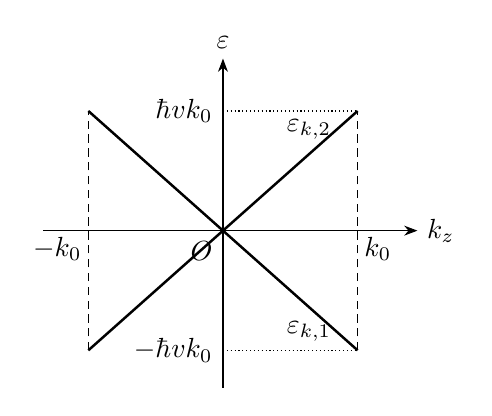
\begin{tikzpicture}[scale=0.95,>=Stealth,line width=0.9pt]
  % 座標軸
  \draw[line width=0.4pt,->] (-2.4,0) -- (2.6,0) node[right] {$k_z$};
  \draw[line width=0.4pt,->] (0,-2.1) -- (0,2.3) node[above] {$\varepsilon$};
  \node[below left] at (0,0) {$O$};

  % バンド分散 epsilon_{k,2} = hbar v |k_z|, epsilon_{k,1} = -hbar v |k_z|
  \draw (-1.8,1.6) -- (0,0) -- (1.8,1.6);
  \draw (-1.8,-1.6) -- (0,0) -- (1.8,-1.6);

  % 境界線 k_z = +/- k_0
  \draw[line width=0.4pt,densely dashed] (-1.8,-1.6) -- (-1.8,1.6);
  \draw[line width=0.4pt,densely dashed] ( 1.8,-1.6) -- ( 1.8,1.6);
  \node[below left,inner sep=2pt] at (-1.8,0) {$-k_0$};
  \node[below right,inner sep=2pt] at ( 1.8,0) {$k_0$};

  % ラベル
  \node[above] at (1.15,1.08) {$\varepsilon_{k,2}$};
  \node[below] at (1.15,-1.08) {$\varepsilon_{k,1}$};
  \node[left] at (0,1.6) {$\hbar v k_0$};
  \node[left] at (0,-1.6) {$-\hbar v k_0$};
  \draw[line width=0.4pt,densely dotted] (0,1.6) -- (1.8,1.6);
  \draw[line width=0.4pt,densely dotted] (0,-1.6) -- (1.8,-1.6);
\end{tikzpicture}
\end{document}
